\chapter{Resultaten}
Hier wordt besproken hoe het uitgewerkte aanbevelingssysteem scoort op de drie belangrijke pijlers: nauwkeurigheid, privacy en performantie.
\section{Privacy}
Deze oplossing biedt veruit de beste privacybescherming uit al de besproken mogelijkheden. Beide servers doen het merendeel van de berekeningen in het ge\"encrypteerd Paillier- of DGKdomein. In de gevallen waar een server rekent met plaintext is deze dermate verstoord zodat deze server de originele waarde niet kan kennen. Het Pailliercryptosysteem en het DGKsysteem worden als semantisch veilig beschouwd. Dit betekent dat het niet \emph{feasible} of computationeel haalbaar is dat er extra informatie kan gehaald worden over de plaintext uit de ciphertext. Homomorfische systemen als Paillier en DGK kampen wel met het probleem dat een aanvaller die een \emph{man-in-the-middle attack} uitvoert de plaintekst kan vermenigvuldigen met een gewenste waarde en kan sturen naar de ontvanger. De aanvaller kan de waarden dan wel niet lezen, hij kan ze verstoren en een geldige waarde sturen naar de ontvanger. Dit kan opgelost worden met behulp van een extra hashwaarde te gebruiken \cite{yi:homomorphic} in ruil voor extra processorgebruik en dataverkeer. Dit werd niet opgenomen in de oplossing aangezien de cryptografische berekeningen op zich al veel serverberekeningen vragen en de twee servers hoogstwaarschijnlijk in een LAN verbonden zijn waar de kans op een dergelijke inbreuk kleiner is. Het privacyniveau ligt zelfs hoger dan in \cite{ZErkinDyn} aangezien de gebruiker hier zijn ratings in bulk doorstuurt en de server dus geen idee heeft welke items een gebruiker beoordeeld heeft. De gebruiker moet er wel op vertrouwen dat (1) de twee servers vertegenwoordigd worden door aparte partijen en dat (2) ze beiden het protocol in volgorde uitvoeren. Beide kunnen gegarandeerd worden indien de controleserver vertegenwoordigd wordt door de overheid. Deze kan de volgorde van het protocol in het oog houden.
\section{Nauwkeurigheid}
De nauwkeurigheid werd onderzocht door de MAE-waarden en RMSE-waarden te berekenen op basis van de MovieLensdatabank met 1682 films, 943 gebruiker en 100.000 ratings. Elke gebruiker heeft dus gemiddeld $100.000/943 =106.0$ beoordelingen gemaakt. Precision en recall vallen in dit geval moeilijk te testen omdat niet kan ingeschat worden hoe relevant een item is voor de persoon die aanbevelingen vraagt. In onze berekeningen wordt 100\% van de gebruikers geselecteerd in het selectieprotocol. De waarden komen dus overeen met een selectie 50\% van 1886 gebruikers genomen uit een veel grotere dataset uit de praktijk. Om de bovengrens te bepalen van de nauwkeurigheid in dit systeem berekenen we de gelijkheidsfactor tussen twee gebruikers op basis van al hun preferences. In de praktijk zal de nauwkeurigheid ook afhangen van het aantal preferences dat er gebruikt wordt en hoe goed deze gekozen zijn. Als test werd er aan het systeem gevraagd 10000 willekeurige testbare aanbevelingen te bepalen met verschillende drempelwaarden voor de gelijkeniswaarde. Met willekeurige testbare aanbevelingen wordt bedoeld dat: 
\begin{enumerate}
\item De aanbevelingen werden gevraagd voor een willekeurige gebruiker voor een willekeurig item.
\item De gebruiker het item zelf heeft beoordeeld. Zo beschikken we over een waarde om de fout op te berekenen op het verwachtte aantal sterren. De aanbevelingen worden natuurlijk berekend zonder de kennis van de echte beoordeelde waarde.
\item Er beoordelingen van dat bepaald item van andere gelijkaardige gebruikers gevonden werden. Hoe hoger de drempelwaarde, hoe minder gebruikers worden opgenomen in het protocol. Indien geen enkele van deze gebruikers deze film beoordeeld heeft, kan geen gemiddelde genomen worden en deze aanbeveling wordt dus als gefaald beschouwd.
\end{enumerate}

\pagebreak
De bedoeling hiervan is om een idee te hebben welke drempelwaarde het best scoort bij onze dataset. We bepalen eerst de MAE, MSE en RMSE-waarden samen met nog een paar andere nuttige waarden:

\begin{center} 
\centering 
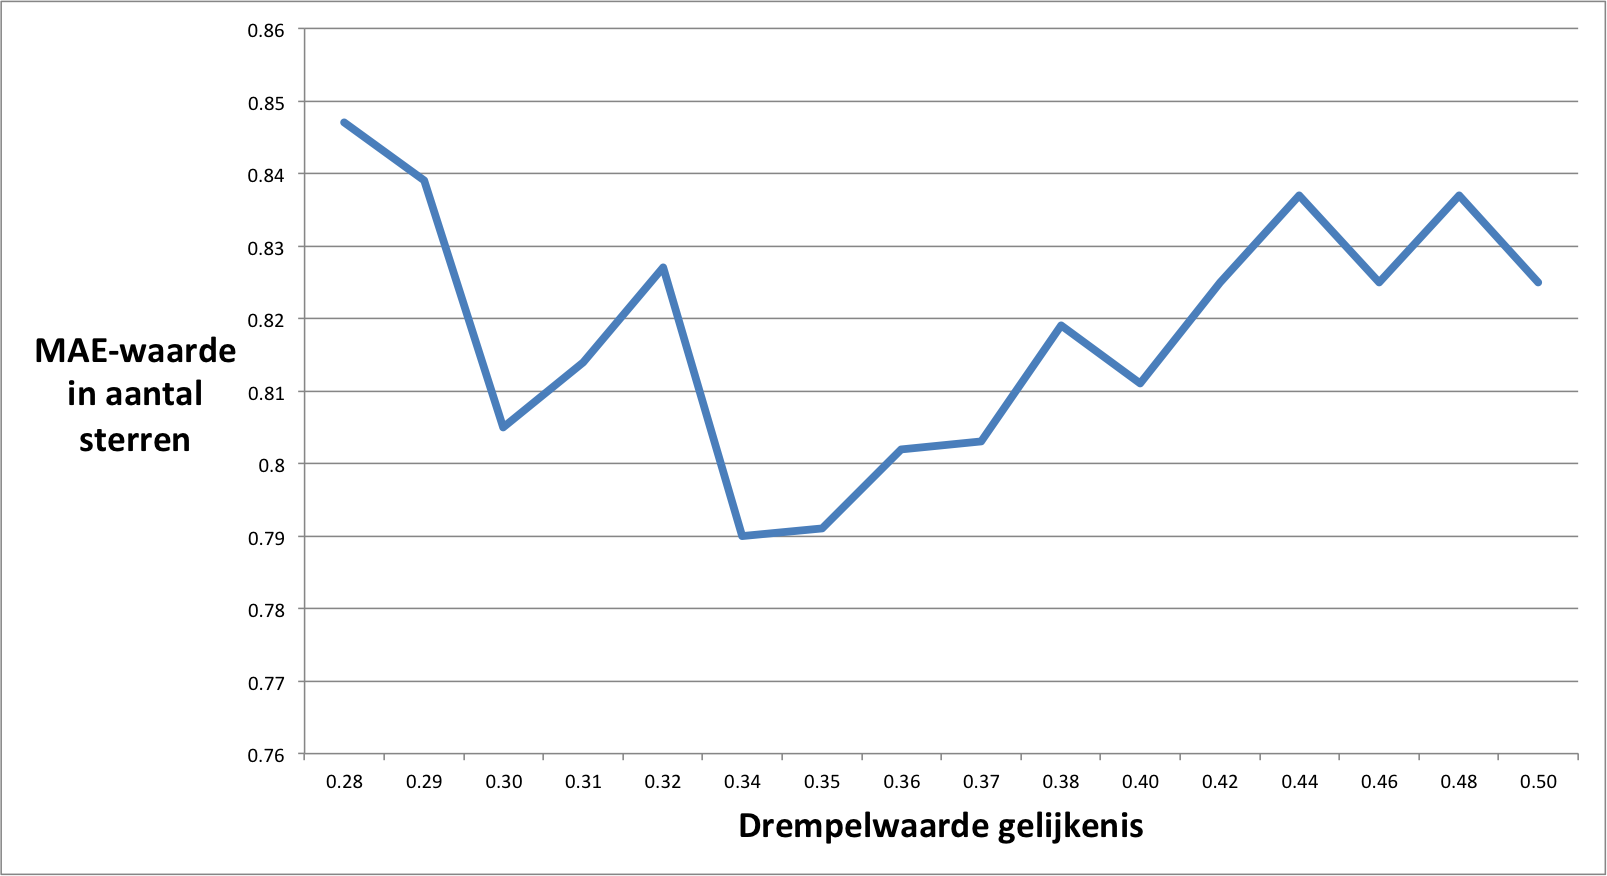
\includegraphics[scale=0.6]{fig/mae}       
\label{Figuur::mae} 
\end{center}
\begin{center} 
\centering 
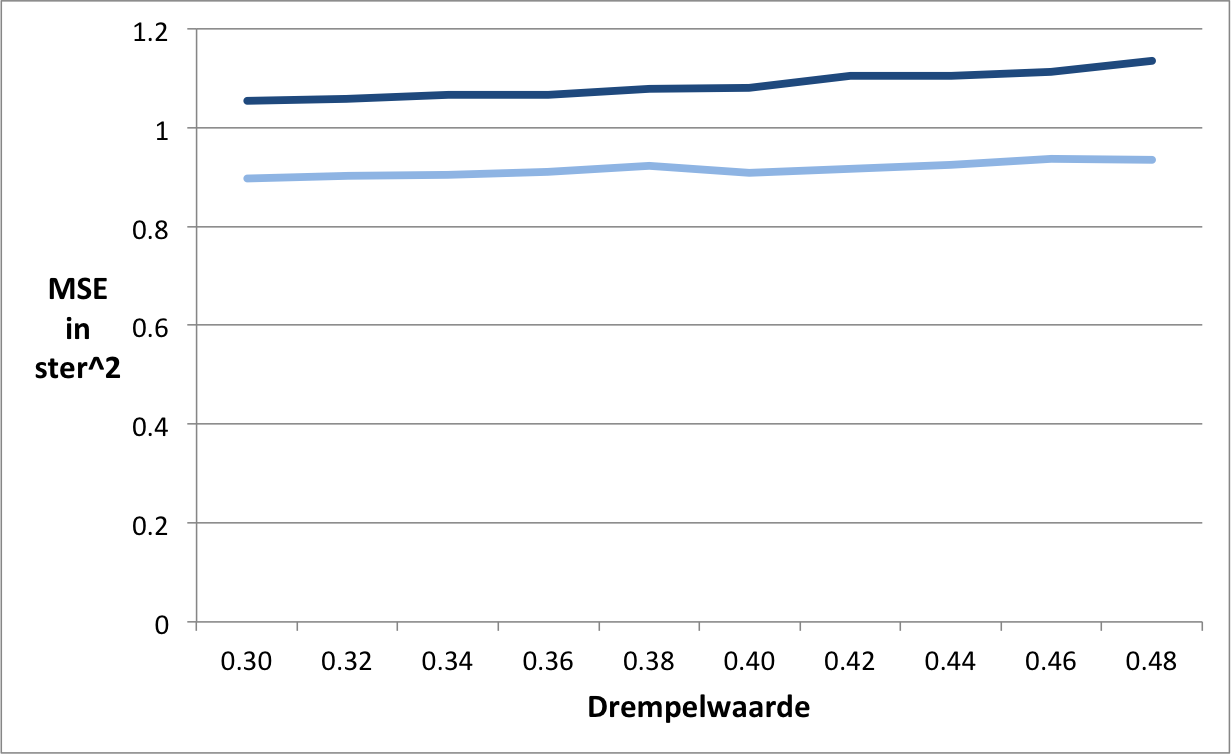
\includegraphics[scale=0.6]{fig/mse}  
    \label{Figuur::mse} 
\end{center}
\begin{center} 
\centering 
 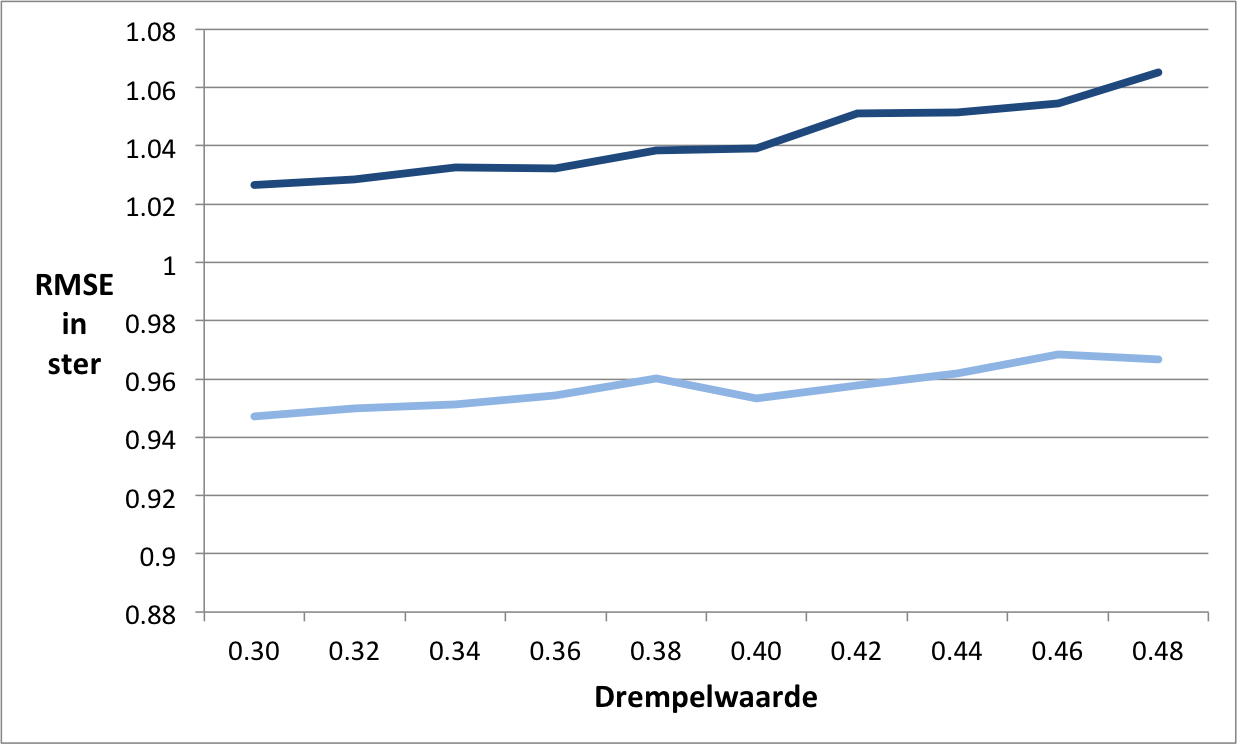
\includegraphics[scale=0.6]{fig/rmse} 
    \label{Figuur::rmse}  
\end{center}

\begin{center} 
\centering 
 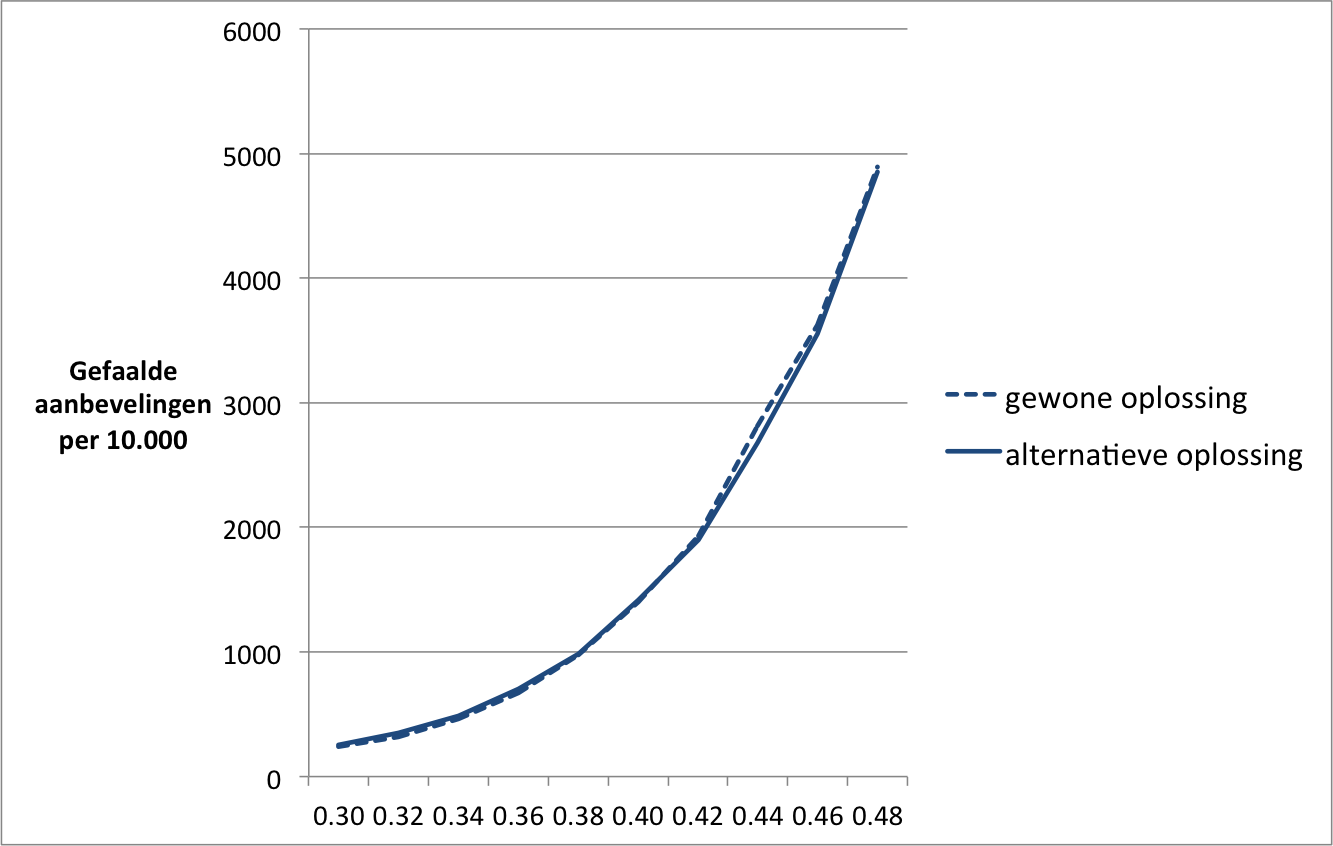
\includegraphics[scale=0.6]{fig/failed}  
    \label{Figuur::failed} 
\end{center}
Voor drempelwaarden groter dan 0.5 werden de aanbevelingen berekend op gemiddeld minder dan 10 beoordelingen van andere gebruikers. De MAE stijgt en er falen veel aanbevelingen, deze waarden zijn dus niet echt nuttig.
\begin{center} 
\centering 
 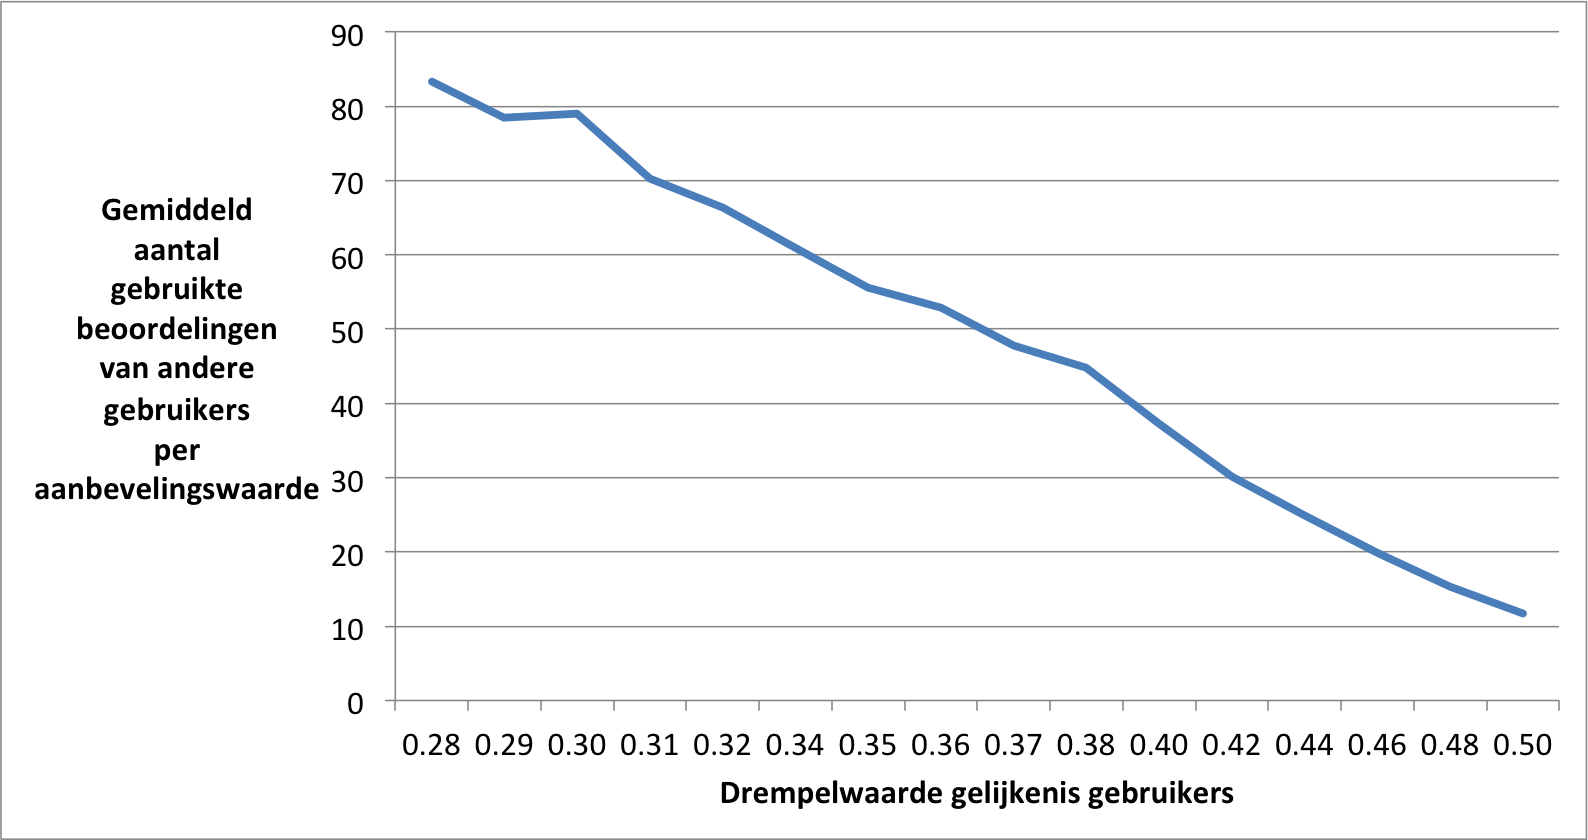
\includegraphics[scale=0.5]{fig/usedratings}     \label{Figuur::usedratings}  
\end{center}

Met een drempelwaarde in de buurt van 0.30 wordt de kleinste MAE, MSE en RMSEwaarden opgemeten in beide methodes. De alternatieve methode scoort duidelijk beter op nauwkeurigheid dan de werkwijze uit \cite{ZErkinDyn}. De MAE-waarde van de alternatieve methode komt in de buurt van 0.74, de oude wijze haalt maar een MAE van 0.82. Er wordt dus beter gescoord dan  de MAE-waarde 0.7964 van de privacyvriendelijke oplossing uit "Svd-based collaborative filtering with privacy\cite{Polat:2005:SCF:1066677.1066860}" besproken in \ref{randomisatie}. In dit artikel werd ook de MAE berekend voor een niet-privacyvriendelijke oplossing: 0.7146. Beide waarden werd berekend op identiek dezelfde dataset van MovieLens. Het verschil van de bekomen MAE 0.74 met de MAE van de niet-privacyvriendelijke methode 0.7146 is dus 0.0254 ster. Er wordt dus niet veel aan nauwkeurigheid ingeboet.
\section{Performantie}
\subsection{Het mobiele toestel}
Het mobiel \emph{device} moet het meeste werk leveren als de gebruiker zijn profiel uploadt. Dan encrypteert het toestel niet alleen de voorkeuren en de beoordelingen van de gebruiker, maar ook een nulwaarde voor de items die niet beoordeeld zijn. Dit gebeurt zodat de service provider niet weet welke items beoordeeld werden. Een andere optie is ook telkens een paar random items uit te kiezen en de nulwaarden hiervan mee te sturen. Het is hierbij wel mogelijk dat alle random items in een bepaalde groep liggen, waardoor de service provider toch smaken kan afleiden. Deze methode is dus $O(N+S)$ waarbij N staat voor het aantal items en S voor het aantal preferences.
In de praktijk komt dit overeen met 1,52 seconden op het testtablet \footnote{Samsung Galaxy Tab4 (7.0) Wi-Fi op Android 4.4.2} als er een richtwaarde genomen wordt van 30 preferences. 

\subsection{De aanbevelingsserver en de controleserver}
Server 1 en 2 moeten zware berekeningen verrichten en veel informatie over en weer sturen. Dit is vooral dankzij het multiplicatieprotocol en het drempelprotocol. De performantie van het zwaarste protocol is $O(N(S+l^2))$ met $l$ het aantal bits van een ge\"encrypteerde waarde. In de praktijk komt het aanvragen van voorspellingswaarden van alle 1682 items voor \'e\'en gebruiker op onze testserver\footnote{MacBook Pro 4 GB RAM 2.4 GHZ i7 processor} overeen met een tijd van 7 minuten 26 seconden bij 30 preferences. Achteraf gezien werd de communicatie tussen de servers beter op een lager protocolniveau ge\"implementeerd dan het HTTP-protocol om tijd te winnen. Door het feit dat de gebruiker voor alle items zijn al dan niet ingevulde beoordelingen doorstuurt, werd de databank ook 15 keer groter. Dit zou beter vermeden zijn door als gebruiker enkel maar beoordelingen voor een aantal slim gekozen items zou doorsturen zoals besproken in \ref{voor_aanvraag}. Er zijn daarbuiten waarschijnlijk ook nog mogelijkheden om de oplossing te optimaliseren op dit gebied.